\documentclass[spanish,a4paper,12pt,twoside]{report}

% MAIN CONFIGURATION
\usepackage[top = 2.5cm, bottom = 3cm, left = 4cm, right = 2cm]{geometry}

\usepackage{algorithm,algorithmic}
% \usepackage[euler]{textgreek}
\usepackage{mathtools}
\usepackage{graphicx}
\usepackage[hidelinks]{hyperref}
\usepackage{indentfirst}
\usepackage[justification=centering]{caption}
\captionsetup[figure]{
  format = hang,
  name = Fig.,
  singlelinecheck = off,
  labelfont = small,
  font = small
}
\setcounter{figure}{0}
\renewcommand{\thefigure}{\arabic{figure}}
\usepackage{lipsum}
\usepackage[spanish]{babel}
\usepackage[T1]{fontenc} % Font type.
\usepackage{titlesec}
\titleformat{\chapter}[display]{\normalfont\bfseries}{}{0pt}{\Huge}
\usepackage[utf8]{inputenc}
\setlength{\parskip}{0.5cm}
\titlespacing{\paragraph}{0pt}{0pt}{0.1cm}[]

% CONTENT
\begin{document}
  \pagenumbering{Roman}
  \begin{titlepage}
    \newcommand{\HRule}{\rule{\linewidth}{0.5mm}}
    \begin{center}
      
\includegraphics[width = 2.25cm]{resources/FACINFO}
      \hspace{8cm}
      
\includegraphics[width = 2cm]{resources/logoupm.png}
      \\[1cm]

      \textsc{\Large Escuela Técnica Superior de Ingenieros Informáticos}
      \\[0.5cm]
      \textsc{\large Universidad Politécnica de Madrid}
      \\[3cm]

      \HRule \\[0.4cm]
      {\huge \bfseries Sistema evolutivo híbrido para la construcción de Redes de Neuronas}
      \HRule \\[4cm]
    
      \textsc{\LARGE Trabajo Fin de Máster}\\[0.5cm]
      \textsc{\Large Máster Universitario en Inteligencia Artificial}\\[3cm]
    \end{center}
    \begin{flushright}
      \large AUTOR: Carlos Vázquez Losada \\TUTOR: Daniel Manrique Gamo
      \\[2.1cm]
    \end{flushright}
    \begin{center}
      {{20 de julio de 2019}}
    \end{center}
    \vfill
  \end{titlepage}
  \newpage\cleardoublepage

  \chapter{\vspace{-3cm}{\LARGE Agradecimientos}}
  \vspace{-1cm}
    Deseo expresar mi agradecimiento, en primer lugar, a Daniel, un investigador incansable y un profesor excepcional. Gracias por dedicarme tu tiempo y adaptarte a mis horarios, y gracias por despertar en mi el interés en la Computación Evolutiva con tus clases y con tu implicación.\par
    A mis padres, Isabel Losada y Fco. Javier Vázquez, por su amor, comprensión y por su apoyo incondicional en todo aquello que me he propuesto.\par
    A Cristina, espectadora de mis éxios y mi acompañante. Siempre sabes que decir y cómo complementarme. Te quiero.
  \vfill
  \newpage\cleardoublepage
  
  \chapter{\vspace{-3cm}{\LARGE Resumen}}
  \vspace{-1cm}
  Este Trabajo de Fin de Máster consiste en estudiar la idoneidad de la Computación Evolutiva para la generación de Redes de Neuronas Artificiales. En concreto, en un estudio de la Programación Genética y si el entrenamiento parcial de las redes candidatas es o no suficiente para resolver estos problemas frente al entrenamiento total de las mismas. \par
  La Programación Genética es una técnica evolutiva que se utiliza en problemas de optimización cuyas soluciones son programas informáticos. La Programación Genética Guiada por Gramáticas extiende las posibilidades de la Programación Genética tradicional con la introducción de las gramáticas, que permiten crear individuos sintácticamente válidos. \par
  Estas gramáticas permiten la confección de arquitecturas de Redes de Neuronas Artificiales que son válidas, dado cualquier número de neuronas en la capa de entrada y en la capa de salida. El resultado de una ejecución nos devolverá la arquitectura de red que mejor se amolde al problema dado, teniendo en cuenta las propias peculiaridades de la gramática utilizada. El objetivo es determinar si el entrenamiento parcial de estas redes da resultados lo más similares posibles al del entrenamiento total, ya que es bastante ineficiente y tardío. \vfill
  \newpage\cleardoublepage
  
  \chapter{\vspace{-3cm}{\LARGE Summary}}
  \vspace{-1cm}
  This Master Thesis Dissertation consists in a research about how appropiate is to use Evolutionary Computation for creating Artificial Neural Networks. A technique of Evolutionary Computation is used for this purpose; Grammar-Guided Genetic Programming. It will be used for looking the best Artificial Neural Network for a concrete dataset, by checking both partially and fully trained networks. \par
  Genetic Programming is an evolutionary technique (it is inspired by biology as Evolutionary Computation does) and it is used for solving optimization problems whose solution is a computer program. The Grammar-Guided Genetic Programming extends Genetic Programming by adding grammars, that allow to create valid individuals. \par
  These grammars allow creating Neural Network architectures that are all valid, given any number of neurons in both input and output layers. The result of an execution would be the architecture that best fixes (in terms of accuracy) the given data.
  \vfill
  \newpage\cleardoublepage
  
  \newpage\cleardoublepage
  \pagenumbering{arabic}
  
  \chapter{\vspace{-3cm}{\LARGE 1. Introducción}}
  \vspace{-1cm}
  La optimización matemática estudia un tipo concreto de problemas donde se desea elegir el mejor entre un conjunto de elementos. El problema clásico (Boyd and Vandenberghe, 2004) consiste en maximizar o minimizar una función objetivo que representa o mide la calidad de las decisiones. Además, esta función está sujeta a un conjunto de restricciones que acotan el espacio de soluciones. \par
  Para resolver estos problemas, existen algoritmos de optimización, métodos iterativos y heurísticas. Uno de los primeros algoritmos de optimización es el algoritmo de Simplex (Dantzig, 1990). Los métodos iterativos buscan la convergencia hacia una solución determinada. Un ejemplo es el Método de Newton (Nocedal et al., 1999). Las heurísticas (Polya, 1945), en cambio, aproximan la solución en el caso de que previamente no haya habido convergencia. \par
  La Computación Evolutiva es una familia de heurísticas inspiradas en la propia evolución biológica de los seres vivos para la resolución de problemas de optimización. En concreto, la Programación Genética (Koza, 1992) surge por la necesidad de extender la optimización para involucrar programas informáticos. \par
  Las Redes de Neuronas Artificiales son técnicas de Aprendizaje Automático (Samuel, 1959) inspiradas en las redes de neuronas propias de los seres vivos. El objetivo de este modelo es la resolución de problemas tal y como lo hace el cerebro humano. Son especialmente utilizadas en los ámbitos de Visión Artificial (Roberts, 1965) y en el Reconocimiento de Voz (Waibel et al., 1989), aunque también son ampliamente usadas para problemas de Aprendizaje Supervisado básicos como los conformados por información proveniente de ficheros, y es en este tipo de clasificación en la que se centra este trabajo. \par
  La Computación Evolutiva y las Redes de Neuronas Artificiales, ambas inspiradas en la biología, no son opuestas sino que se complementan. La Computación Evolutiva permite resolver problemas de optimización y búsqueda, mientras que las Redes de Neuronas Artificiales son indicadas para el Aprendizaje Automático. La Programación Genética supuso una alternativa a la búsqueda de la mejor Red de Neuronas Artificiales, ya que, antiguamente, la selección de la arquitectura se basaba en la experiencia previa, y en la preba y el error. \par
  El objetivo principal de este trabajo es estudiar la idoneidad de la Computación Evolutiva para la generación de Redes de Neuronas Artificiales. Para ello, se utilizará una de las técnicas de esta familia de heurísticas, la Programación Genética Guiada por Gramáticas, para tal fin. En concreto, se establecen varios objetivos:
  \begin{enumerate}
    \item Determinar si el entrenamiento parcial de los individuos (redes) de un programa genético para buscar la mejor arquitectura de Red de Neuronas Artificiales es comparable con el entrenamiento total y se obtienen resultados idénticos, para ahorrar así grandes tiempos de ejecución.
    \item Implementar un Programa Genético que lidie con Redes de Neuronas y que permita el estudio propuesto.
    \item Probar la gramática con ejemplos diversos para realizar un estudio más exhaustivo sobre ella.
  \end{enumerate} \par
  Este documento se estructura en siete secciones después de esta introducción. Las dos primeras se centran en la \emph{Computación Evolutiva} y en las \emph{Redes de Neuronas Artificiales}, respectivamente. La tercera sección trata sobre la \emph{construcción de Redes de Neuronas}, seguida del \emph{planteamiento del problema}, en la que se describe con profundidad el propósito de este trabajo y la necesidad real de él. A esta sección le sigue la \emph{solución propuesta}, que contiene la metodología y el procedimiento seguido, exponiendo los \emph{resultados} obtenidos en la séptima sección. Finalmente, el trabajo finaliza con las \emph{conclusiones y líneas futuras} propuestas. \par
  
  \chapter{\vspace{-3cm}{\LARGE 2. Computación Evolutiva}}
  \vspace{-1cm}
  La Computación Evolutiva comprende un conjunto de técnicas para la resolución de problemas de búsqueda y optimización inspiradas en la evolución biológica de los seres vivos. En este capítulo se ofrecen, en primer lugar, un resumen de la \emph{historia} de la Computación Evolutiva. Seguidamente, una \emph{definición} sobre esta rama de estudio y que finaliza hablando sobre la \emph{Programación Genética} y la \emph{Programación Genética Guiada por Gramáticas}.
  \section*{\Large 2.1. Historia}
  La Computación Evolutiva surge con los trabajos de Box (Box, 1957),  Friedberg (Friedberg, 1958, 1959) y Bremermann (Bremermann, 1962). Sin embargo, no se consiguieron grandes avances debido a la pobre metodología todavía sin desarrollar y a las limitaciones computacionales de la época. \par
  Algunos años después surgen los primeros desarrollos metodológicos en una década de destacable logro científico. El trabajo de Fogel (Fogel et al., 1966) sienta las bases de la Programación Evolutiva (\emph{evolutionary programming}) y el de Holland (Holland, 1967) las de los Algoritmos Genéticos (\emph{genetic algorithms}). También, en esa misma época, las Estrategias Evolutivas (\emph{evolution strategies}) fueron introducidas por Rechenberg (Rechenberg, 1965) y Schwefel (Schwefel, 1965). \par
  Una década después de los primeros descubrimientos, alrededor de los años 80, los avances computacionales permitieron aplicar las técnicas evolutivas descubiertas para resolver problemas de optimización del mundo real. En esa misma década, los estudios de Cramer (Cramer, 1985) y Koza (Koza, 1988) desembocaron en la aparición de una nueva técnica perteneciente a la Computación Evolutiva: la Programación Genética (\emph{genetic programming}). Pocos años después, la Programación Genética contaba con más de 10.000 artículos publicados (Hu et al., 2014). Pocos años después ya habría cerca de 10.000 publicaciones sobre esta peculiar heurística. También se sucedieron una gran cantidad de conferencias internacionales y talleres centrados en aspectos teóricos de los Algoritmos Genéticos (Grefenstette, 1985, 1987; Schaffer, 1989), entre muchos otros. Estos años destacaron también por la aparición de otras técnicas de Computación Evolutiva como la Vida Artificial (\emph{artificial life}) abreviada muy comúnmente como \emph{A-Life} (Langton, 1986), los Sistemas Inmunitarios Artificiales (\emph{artificial immune systems}) (Farmer et al., 1986), la Inteligencia de Enjambre (\emph{swarm intelligence}) (Beni and Wang, 1989) y los Algoritmos Meméticos (Moscato, 1989). \par
  Hacia 1990, era innegable admitir que parte de la comunidad científica del mundo ponía sus ojos en la Computación Evolutiva. A las conferencias anteriormente expuestas le siguieron las cuatro conferencias de IEEE sobre Computación Evolutiva, que asentaron esta rama de estudio como una de las articulaciones de la Inteligencia Artificial y herramienta indispensable para la resolución de problemas de optimización y búsqueda en el ámbito académico y empresarial. La conferencia de Programación Genética (Koza et al., 1996) tuvo gran éxito y aceptación, a la cual le siguieron otras conferencias sobre el mismo ámbito, como la EuroGP (Banzhaf, 1998). Destacaron también conferencias sobre desarrollos metodológicos sobre los Algoritmos Genéticos (Rawlins, 1991; Whitley, 1993; Vose, 1995), que se consolidó como la técnica de Computación Evolutiva más destacable. Esta década se cierra con la llegada de nuevas técnicas de Computación Evolutiva: los Algoritmos Culturales (\emph{cultural algorithms}) (Reynolds, 1994), la Evolución Diferencial (\emph{differential evolution}) (Storn, 1996; Storn and Price, 1997) y la Evolución Gramatical (\emph{grammatical evolution}) (Ryan et al., 1998), además de la aparición de una variante de la Programación Genética, la Programación Genética Guiada por Gramática (Whigham \par
  A estas casi cuatro décadas de gran logro científico le siguieron dos más de un impecable desarrollo metodológico. En estos años destacaron los estudios sobre los Algoritmos Genéticos (Deb et al., 2002; Hassan et al., 2005; Pezzella et al., 2008), entre muchos otros, además de la aparición de nuevas heurísticas como la Búsqueda Armónica (\emph{harmony search}) (Geem et al., 2001) o los Algoritmos Genéticos Basados en Humanos (\emph{human based genetic algorithms}) (Kosorukoff, 2001). Otras técnicas evolutivas también tuvieron su amplio desarrollo metodológico y crecimiento teórico (Couchet and Manrique, 2006; De Araujo and Tavares, 2014; Beni, 2004).
  \section*{\Large 2.2. Funcionamiento general}
  La Computación Evolutiva se fundamenta en la evolución biológica y cuenta con un conjunto de heurísticas para la resolución de problemas de búsqueda y optimización. Cada una de ellas sirve para un tipo concreto de problemas de este ámbito, no asegurando su eficacia si se utiliza en otro dominio. \par
  La evolución biológica se basa en la Teoría de la Evolución de Darwin (Darwin, 1959), donde los individuos son los protagonistas. Estos individuos viven en poblaciones, de tal forma que se produce una evolución conjunta de la población mediante la aplicación de operadores evolutivos tales como la selección, el reemplazo, el cruce y la mutación. \par
  Para la Computación Evolutiva, los individuos son las soluciones candidatas al problema de búsqueda u optimización dado. La población se compone del conjunto de individuos base y de la que parte la ejecución del algoritmo. Sobre esta población se aplican los operadores evolutivos (referidos en este ámbito como operadores genéticos) anteriormente mencionados, con el objetivo de que se produzca una mejora y un acercamiento gradual hacia la solución óptima en cada generación. Teóricamente, se espera que tras un número finito de generaciones, la población haya convergido hacia la solución óptima al problema dado. En la práctica, puede que sea conveniente limitar este número de generaciones por las capacidades computacionales limitadas que hoy en día existen, y la población llegue hasta un cierto grado de optimalidad. \par
  Este proceso se lleva a cabo conformando el Ciclo Evolutivo (Koza, 1996) que se repite hasta que finalmente se cumple la condición de parada.
  \begin{figure}[H]
    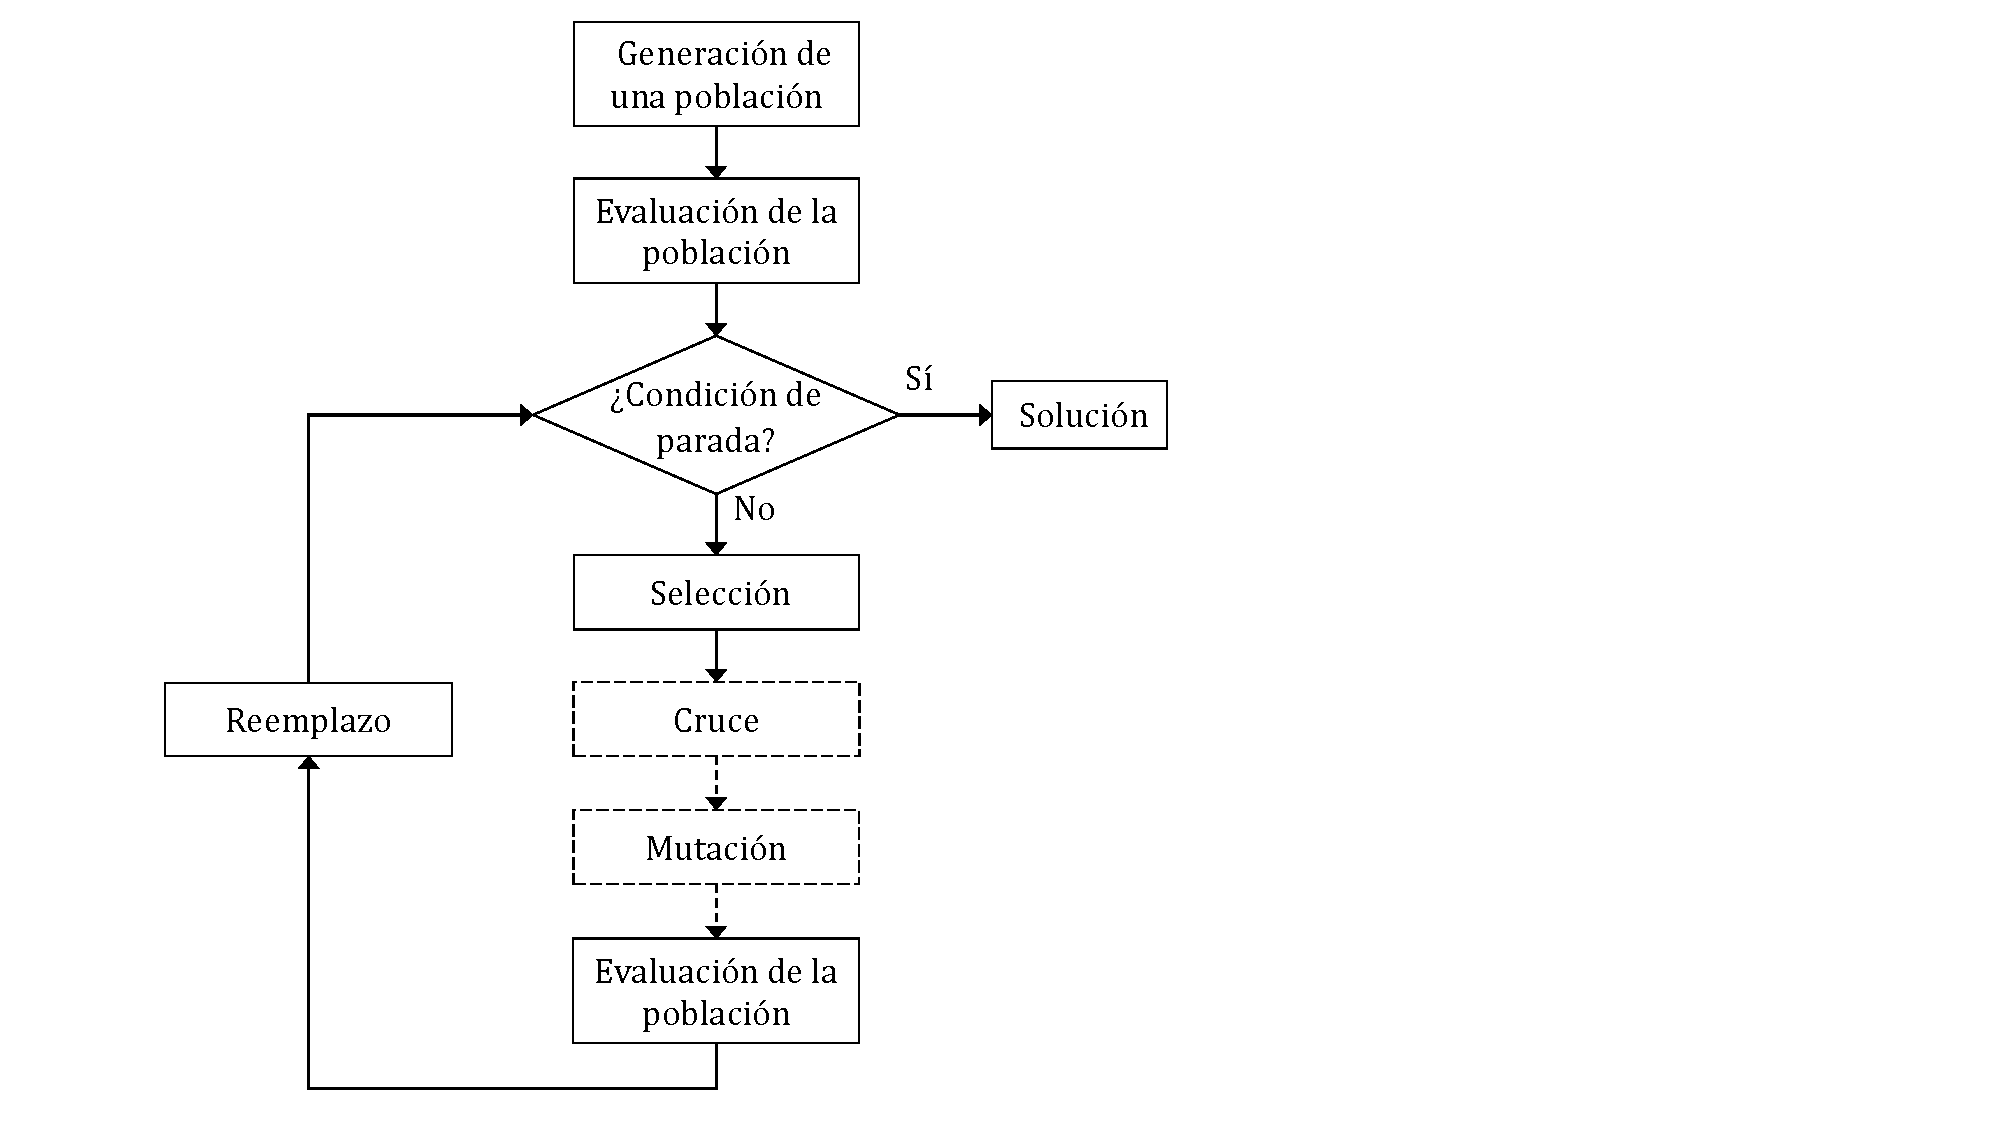
\includegraphics[width = 1\textwidth]{resources/Fig1.pdf}
    \caption{Ciclo Evolutivo que rige el desarrollo de los algoritmos en la Computación Evolutiva.}
    \label{fig:1}
  \end{figure}
  En Fig. \ref{fig:1} se puede apreciar este Ciclo Evolutivo. Todo comienza con una población inicial, que se corresponderá con un conjunto de individuos $Z$ de tamaño $\alpha$ que serán seleccionados del espacio de búsqueda $E$, que es la codificación, completa o no, dependiendo del alfabeto $A$ utilizado en este proceso, del espacio de soluciones $S$. Esta codificación se lleva a cabo mediante una función de codificación $\Omega$. La elección del alfabeto $A$ es fundamental, ya que, dependiendo de su precisión, puede que haya individuos del espacio $S$ que no tengan representación en el espacio $E$, y si es una solución potencialmente buena (incluyendo la óptima), entonces el proceso evolutivo nunca la encontrará. \par
  Tras la conformación de la población inicial (a partir del espacio de búsqueda $E$), se evalúa, por medio de una función de evaluación (\emph{fitness function}), a sus individuos para determinar su grado de adaptación, de tal forma que un valor muy alto implicará que ese individuo tiene un grado mejor de adaptabilidad que otro cuyo valor sea más bajo (y que, por tanto, tendrá más probabilidades de mantenerse en la población inicial). Para este proceso de evaluación, en algunas ocasiones, hará falta decodificar a los individuos, por lo que se aplicará la función de decodificación $\Omega^{-1}$. \par \vfill
  Tras el proceso de generación de la población inicial $Z$, se determina si se cumple la condición de parada (\emph{stop condition}), que es un compendio de condiciones lógicas que detiene el ciclo evolutivo si se cumple, y en caso contrario, continúa. Las condiciones siguen un estricto e inalterable orden que permite el correcto funcionamiento de este proceso.
  \begin{enumerate}
    \item Algún individuo de la población contiene la solución óptima al problema.
    \item La población ha convergido (a una solución óptima o no).
    \item Se ha alcanzado el número máximo de generaciones.
  \end{enumerate} \par
  En el primer caso, la ejecución finaliza devolviendo el individuo óptimo y, por tanto, encontrando la solución. Si la población converge sin haber encontrado antes un individuo óptimo (la población evoluciona después de comprobar la condición de parada, por lo que puede que haya convergido a la optimalidad después de la comprobación previa), entonces finaliza devolviendo cualesquiera de los individuos de la misma. Si no se cumple ninguna de estas dos condiciones, entonces se comprueba si se han superado el número de generaciones máximas determinadas por el usuario. En caso afirmativo, finaliza devolviendo el mejor individuo (no óptimo) de la población. En el caso de que no se cumpla ninguna condición de parada, el algoritmo continúa. \par
  Después, si la población no ha sufrido una evolución en la generación anterior, entonces se aplican los operadores genéticos de selección (\emph{selection}), cruce (\emph{crossover}) y mutación (\emph{mutation}) sobre los individuos. Tras aplicar estos tres operadores, se evalúa la población resultante y se comprueba si se cumple la condición de parada. Si a la población si se le han aplicado estos operadores, entonces se aplica solo el operador genético de reemplazo (\emph{replace}), que generará una nueva población y el proceso se repetirá hasta que se cumpla la condición de parada. \par
  Como se ha mencionado, existen un total de cuatro operadores genéticos que actúan, dependiendo del tipo, sobre la propia población $Z$ o el espacio de búsqueda $E$. Estos operadores se definen como:
  \begin{itemize}
    \item Selección. Es el operador encargado de elegir a los individuos de $Z$ que se cruzarán para generar otros nuevos. La cantidad de individuos seleccionados $\pi$ coincidirá con la cantidad de descendientes producidos. El fundamento radica que en la naturaleza, aquellos individuos mejor adaptados tendrán una probabilidad de reproducción mayor frente aquellos que no lo estén. Por tanto, una implementación tradicional consiste en seleccionar con mayor probabilidad a los mejor adaptados, pero hay otras elitistas que seleccionan solo a los $\pi$ mejor adaptados, desechando a los peores individuos.
    \item Cruce. Los individuos seleccionados por el operador anterior acceden al \emph{mating pool}. Estos individuos reciben el nombre de progenitores (\emph{progenitors}) y que se reproducirán para conformar su descendencia (\emph{offspring}). Normalmente, los progenitores se reproducen por parejas, conformando 2 descendientes. A rasgos del ciclo, este operador es opcional para muchos individuos de la población, ya que no todos son seleccionados. Este operador se aplica sobre los individuos de la población, pero permite generar otros individuos nuevos del espacio $E$ y que no estaban codificados en ningún otro individuo de la población, aumentando la diversidad.
    \item Mutación. Con cierta probabilidad (normalmente entre un 5 y un 10\%), un individuo de la población $Z$ experimenta cambios en su genoma (\emph{genome}). Esto permite aumentar la diversidad de la población al generar otra posible solución potencial (puede ser peor o mejor que el individuo previo a la mutación).
    \item Reemplazo. Este operador selecciona a los $\alpha$ individuos que formarán parte de la siguiente generación, es decir, de la nueva población si no se cumple la condición de parada después de aplicar los tres operadores anteriores. Hay muchas políticas de reemplazo, pero el fin común es producir la mejora gradual de los individuos generación a generación (o lo que es lo mismo, sustituir las peores soluciones con otras mejores).
  \end{itemize} \par
  Se puede apreciar que los operadores resultan indispensables para el desarrollo y mejora de la población y su llegada hacia la solución óptima. En concreto, el cruce es el máximo responsable del proceso evolutivo, ya que es el encargado de generar nueva descendencia, tratando de seleccionar los mejores genes de cada progenitor. \par
  Según los operadores que se seleccionen o implementen, la técnica evolutiva realizará labores de exploración (\emph{exploration}) o de explotación (\emph{exploitation}). La exploración consiste en muestrear regiones desconocidas en el espacio de búsqueda $E$ donde pueden encontrarse las soluciones óptimas. La explotación trata de mejorar al individuo más destacado, acortando la búsqueda de la solución óptima en una búsqueda local. Por tanto, estos operadores (y en especial el operador de cruce) se deben comportar de forma explotativa en las primeras generaciones, ya que hay una gran diversidad y de otra forma se produciría una convergencia muy lenta. Sin embargo, a medida que la población va convergiendo hacia una solución, es necesario que los operadores exploren, es decir, escapen hacia otras regiones de búsqueda. \par
  La mayor parte de las heurísticas que forman parte de la Computación Evolutiva siguen el patrón descrito, salvo aquellas que, debido al problema que abordan, tienen una estructura que difiere al resto.
  
  \section*{\Large 2.3. Programación Genética}
  La Programación Genética (Cramer, 1985; Koza, 1988) es una heurística de la familia de la Computación Evolutiva y que permite resolver problemas de búsqueda y de optimización cuyas soluciones son programas informáticos.

  \section*{\Large 2.3. Programación Genética Guiada por Gramáticas}
  
  \chapter{\vspace{-3cm}{\LARGE 3. Redes de Neuronas Artificiales}}
  
  \chapter{\vspace{-3cm}{\LARGE 4. Construcción de Redes de Neuronas}}
  
  \chapter{\vspace{-3cm}{\LARGE 5. Planteamiento del problema}}
  
  \chapter{\vspace{-3cm}{\LARGE 6. Solución propuesta}}
  
  \chapter{\vspace{-3cm}{\LARGE 7. Resultados}}
  
  \chapter{\vspace{-3cm}{\LARGE 8. Conclusiones y líneas futuras}}
  \vfill
  
  \begin{thebibliography}{00}
  \vspace{-1cm}
  \makeatletter
  \def\@biblabel#1{}
  \let\old@bibitem\bibitem
  \def\bibitem#1{\old@bibitem{#1}\leavevmode\kern-\bibindent}
  \makeatother
  
  \bibitem{Banzhaf1998} Banzhaf, W., Poli, R., Schoenauer, M. and Fogarty, T.C. (1998). \emph{Genetic Programming}.
  \bibitem{Beni1989} Beni, G. and Wang, J. (1989). Swarm intelligence in cellular robotic systems. \emph{Proceedings5 of the NATO Advance Workshop on Robots and Biological Systems}. 102:703-712.
  \bibitem{Beni2004} Beni, G. (2004). From Swarm Intelligence to Swarm Robotics. \emph{International Workshop on Swarm Robotics}. 3342:1-9.
  \bibitem{Boyd2004} Boyd, S. and Vandenberghe, L. (2004). Convex Optimization. \emph{Cambridge University Press 2004}: 129.
  \bibitem{Box1957} Box, G.E.P. (1957). Evolutionary operation: A method for increasing industrial productivity. \emph{Journal of the Royal Statistical Society. Series C}. 6(2):81-101.
  \bibitem{Box1969} Box, G.E.P. and Draper, N.P. (1969). \emph{Evolutionary Operation. A method for Increasing Industrial Productivity}.
  \bibitem{Bremermann1962} Bremermann, H.J. (1962). Optimization through evolution and recombination. \emph{Self-Organizing Systems 1962}: 93-106.
  \bibitem{Couchet2006} Couchet, J. and Manrique, D. (2006). Crossover and mutation operations for grammar-guided genetic programming. \emph{Soft Computing}. 11(10):943-955.
  \bibitem{Cramer1985} Cramer, N.L. (1985). A representation for the Adaptive Generation of Simple Sequential Programs. \emph{Proceedings of the First International Conference on Genetic Algorithms and the Applications}: 183-187.
  \bibitem{Dantzig1990} Dantzig, G.B. (1990). Origins of the simplex method. \emph{A history of scientific computing}, pages 141-151.
  \bibitem{Darwin1859} Darwin, C. (1859). \emph{On the Origin of Species by Means of Natural Selection, or Preservation of Favoured Races in the Struggle for Life}. 
  \bibitem{deAraujo2014} De Araujo, A.F. and Tavares, J.M.R.S. (2014). An Artificial Life Model for Image Enhancement. \emph{15th International Conference on Experimental Mechanics}. 41(13):5892-5906.
  \bibitem{Deb2002} Deb, K., Agarwal, S., Pratap, A. and Meyarivan, T. (2002). A Fast and Elitist Multiobjective Genetic Algorithm: NSGA-II. \emph{IEEE Transactions on Evolutionary Computation}. 6(2):128-197.
  \bibitem{Farmer1986} Farmer, J.D., Packard, N.H. and Perelson, A.S. (1986). The Immune System, Adaptation, and Machine Learning. \emph{Physica D: Nonlinear Phenomena}. 22(1): 187-204.
  \bibitem{Fogel1966} Fogel, L.J., Owens, A.J. and Walsh, M.J. (1966). \emph{Artificial Intelligence through Simulated Evolution}.
  \bibitem{Fraser1957} Fraser, A.S. (1957). Simulation of Genetic Systems by Automatic Digital Computers. \emph{Australian journal of biological sciences}. 10:484-499.
  \bibitem{Friedberg1958} Friedberg, R.M. (1958). A learning machine: part I. \emph{IBM Journal of Research and Development}. 2(1):2-13.
  \bibitem{Friedberg1959} Friedberg, R.M., Dunham, B. and North, J.H. (1959). A learning machine: part II. \emph{IBM Journal of Research and Development}. 3(3):282-287.
  \bibitem{Geem2001} Geem, Z.W., Kim, J.H. and Loganathan, G.V. (2001) A New Heuristic Optimization Algorithm: Harmony Search. \emph{Simulation}, 76(2):60-68.
  \bibitem{Grefenstette1985} Grefenstette, J.J. (1985). \emph{Proceedings of the First International Conference on Genetic Algorithms and the Applications} (Hillsdale, NJ: Lawrence Erlbaum).
  \bibitem{Grefenstette1987} Grefenstette, J.J. (1987). \emph{Proceedings of the Second International Conference on Genetic Algorithms and the Applications} (Hillsdale, NJ: Lawrence Erlbaum).
  \bibitem{Hassan2005} Hassan, R., Cohanim, B., de Weck, O. and Venter, G. (2005). A comparison of particle swarm optimization and the genetic algorithm. \emph{46th AIAA/ASME/ASCE/AHS/ASC Structures, Structural Dynamics and Materials Conference}.
  \bibitem{Holland1962} Holland, J.H. (1962). Nonlinear environments permitting efficient adaptation. \emph{Computer and Information Sciences II}: 147-164.
  \bibitem{Hu2014} Hu, T., Banzhaf, W. and Moore, J.H. (2014). The effects of recombination of phenotypic exploration and robustness in evolution. \emph{Artificial Life}. 20(4):457-470.
  \bibitem{Koza1988} Koza, J.R. (1988). Non-Linear Genetic Algorithms for Solving Problems. \emph{University States Patent 4935877}.
  \bibitem{Koza1992} Koza, J.R. (1992). \emph{Genetic Programming 1992} (Cambridge, MA: MIT Press).
  \bibitem{Koza19961} Koza, J.R.(1996). \emph{Genetic Programming: On the Programming of Computers by Means of Natural Selection}  (Cambridge, MA: MIT Press).
  \bibitem{Koza1996} Koza, J.R., Goldberg, D.E., Fogel, D.B. and Riolo, R.L. (1996). \emph{Genetic Programming 1996} (Cambridge, MA: MIT Press).
  \bibitem{Kosorukoff2001} Kosorukoff, A. (2001). Human based genetic algorithm. \emph{2001 IEEE International Conference on Systems, Man and Cybernetics. e-Systems and e-Man for Cybernetics in Cyberspace}: 3464-3469.
  \bibitem{Langton1986} Langton, C.G. (1986). Studying artificial life with cellular automata. \emph{Physica D: Nonlinear Phenomena}. 22(1):120-149.
  \bibitem{Moscato1989} Moscato, P. (1989). On Evolution, Search, Optimization, Genetic Algorithms and Martial Arts - Towards Memetic Algorithms. \emph{Caltech Concurrent Computation Program}: 158-179.
  \bibitem{Nocedal1999} Nocedal, J. and Wright, S.J. (1999). Numerical optimization. \emph{Springer-Verlag}.
  \bibitem{Pezzella2008} Pezzella, F., Morganti, G. and Ciaschetti, G. (2008). A genetic algorithm for the Flexible Job-shop Scheduling Problem. \emph{Computers \& Operations Research}. 35(10):3202-3212.
  \bibitem{Polya1945} Polya, G. (1945). How to Solve It. \emph{Princeton University Press 1945}.
  \bibitem{Rawlins1991} Rawlins, G.J.E. (1991). \emph{Foundations of Genetic Algorithms} (San Mateo, CA: Morgan Kaufmann).
  \bibitem{Rechenberg1965} Rechenberg, I. (1965). Cybernetic Solution Path of an Experimental Problem. \emph{Royal Aircraft Establishment Library Translation 1122}.
  \bibitem{Reynolds1994} Reynolds, R.G. (1994). An Introduction to Cultural Algorithms. \emph{Proceedings of the 3rd Annual Conference on Evolutionary Programming}: 131-139.
  \bibitem{Roberts1965} Roberts, L. (1965). Machine perception of 3D solids. \emph{Optical and Electro-Optical Information Processing}. 9:159-197.
  \bibitem{Ryan1998} Ryan, C., Collins, J.J. and O'Neil, M. (1998). Grammatical Evolution: Evolving Programs for an Arbitrary Language. \emph{Proceedings of the First European Workshop on Genetic Programming}: 83-96.
  \bibitem{Samuel1959} Samuel, A.L. (1959). Some Studies in Machine Learning Using the Game of Checkers. \emph{IBM Journal of Research and Development}. 3(3):210-229.
  \bibitem{Schaffer1989} Schaffer, J.D. (1989). \emph{Proceedings of the Third International Conference on Genetic Algoritms and the Applications} (San Mateo, CA: Morgan Kaufmann).
  \bibitem{Schwefel1965} Schwefel, H-P. (1965). Kybernetische Evolution als Strategie der experimentellen Forschung in der Strömungstechnik.
  \bibitem{Storn1996} Storn, R. (1996). On the usage of differential evolution for function optimization. \emph{Biennial Conference of the North American Fuzzy Information Processing Society}: 519-523.
  \bibitem{Storn1997} Storn, R. and Price, K. (1997). Differential evolution - a simple and efficient heuristic for global optimization over continuous spaces. \emph{Journal of Global Optimization}. 11(4):341-359.
  \bibitem{Vose1995} Vose, M.D. and Whitley, L.D. (1995). \emph{Foundations of Genetic Algorithms 3} (San Francisco, CA: Morgan Kaufmann).
  \bibitem{Waibel1989} Waibel, A., Hanazawa, T., Hinton, G., Shikano, K. and Lang, K.J. (1989). Phoneme recognition using time-delay neural networks. \emph{IEEE Transactions on Acoustics, Speech, and Signal Processing}. 37(3):328-339.
  \bibitem{Whigham1995} Whigham, P.A. (1995). Grammatically-based genetic programming. \emph{Proceedings of the workshop on genetic programming: from theory to real-world applications}: 33-41.
  \bibitem{Whitley1993} Whitley, L.D. (1993). \emph{Foundations of Genetic Algorithms 2} (San Mateo, CA: Morgan Kaufmann).
  \end{thebibliography}
  
\end{document}
